\documentclass[a4paper,9pt]{beamer}
\usetheme{Malmoe}  % Base theme
% Now we try to put MILA's colors
\definecolor{MilaBlue1}{RGB}{78,179,225} % lighter, PMS 306
\definecolor{MilaBlue2}{RGB}{35,154,204} % darker, PMS 639

\setbeamercolor{structure}{fg=MilaBlue2}
\setbeamercolor{title}{fg=MilaBlue1,bg=black}
\setbeamercolor{section in head/foot}{fg=MilaBlue1,bg=black}
\setbeamercolor{subsection in head/foot}{fg=MilaBlue2,bg=white}
\setbeamercolor{frametitle}{fg=white,bg=MilaBlue2}

\setbeamertemplate{footline}[page number]
\usepackage[utf8]{inputenc}
\usepackage{url}
\usepackage{minted}

\usepackage[T1]{fontenc}
\usepackage{inconsolata}

% for copy-pastable ', we need the following
\usepackage{upquote}
\usepackage{textcomp}

%\usepackage{ragged2e}
%\usepackage{multirow}
%\usepackage{fancyvrb}
%\usepackage{color}
\def\imagetop#1{\vtop{\null\hbox{#1}}}

% Standard LaTeX stuff - note the optional abbreviated title being provided

%% ALL that presentation slide are not used! We use a normal frame for that.
\title[Intro to Theano]{Introduction to Theano}
\subtitle{A Fast Python Library for Modelling and Training}
\author[MILA]{Pascal Lamblin}
\institute{%
Montreal Institute for Learning Algorithms (MILA)\\
Université de Montréal}

\date{%
September 25th, 2016, Stanford
}

\setbeamertemplate{navigation symbols}{}


\begin{document}

\begin{frame}[plain]
  \titlepage
  
\includegraphics[width=1in]{MILA_official_2016.png}
  \hfill
  
\includegraphics[width=1in]{UdeM_logo.pdf}
\end{frame}


\subsection*{Introduction}

\begin{frame}{Objectives}
  This session will have 3 parts:
  \begin{itemize}
    \item Introduction to Theano
    \item Hands-on example: ConvNet
    \item Hands-on example: LSTM
  \end{itemize}
  All the material is online at
  \url{github.com/lamblin/bayareadlschool/}

\end{frame}

\begin{frame}{Theano vision}

  Mathematical symbolic expression compiler

  \begin{itemize}
    \item Easy to define expressions
      \begin{itemize}
        \item Expressions mimic NumPy's syntax and semantics
        \item Support for elementary operations (not only neural layers)
      \end{itemize}
    \item Possible to manipulate those expressions
      \begin{itemize}
        \item Substitutions
        \item Gradient, R operator
        \item Stability optimizations
      \end{itemize}
    \item Fast to compute values for those expressions
      \begin{itemize}
        \item Speed optimizations
        \item Use fast back-ends (CUDA, BLAS, custom C code)
      \end{itemize}
    \item Tools to inspect and check for correctness
  \end{itemize}
\end{frame}

\begin{frame}[fragile]{Current status}
  \begin{itemize}
    \item Mature: developed and used since January 2008 (8 years old)
    \item Good user documentation
    \item Active mailing list with participants worldwide
    \item Many contributors from different places
    \item Driven hundreds of research papers
    \item Used to teach university classes
    \item Core technology for Silicon Valley start-ups
    \item Used for research at large companies
  \end{itemize}
  Theano: \url{deeplearning.net/software/theano/}

  Deep Learning Tutorials: \url{deeplearning.net/tutorial/}
\end{frame}

\begin{frame}{Related projects}
  Many libraries are built on top of Theano (mostly machine learning)
  \begin{itemize}
  \item Blocks
  \item Keras
  \item Lasagne
  \item PyMC 3
  \item sklearn-theano
  \item Platoon
  \item Theano-MPI
  \item \ldots
  \end{itemize}
\end{frame}


\section{Symbolic expressions}
\begin{frame}
  \tableofcontents[currentsection]
\end{frame}

\begin{frame}{Overview}
  Theano defines a {\bf language}, a {\bf compiler}, and a {\bf library}.
  \begin{itemize}
    \item Define a symbolic expression
    \item Compile a function that can compute values
    \item Execute that function on numeric values
  \end{itemize}
\end{frame}

\subsection{Declaring inputs}
\begin{frame}[fragile]{Symbolic inputs}
  Symbolic, strongly-typed inputs
  \begin{minted}[fontfamily=tt]{python}
import theano
from theano import tensor as T
x = T.vector('x')
y = T.vector('y')
  \end{minted}

  \begin{itemize}
    \item All Theano variables have a type
    \item For instance \verb|ivector|, \verb|fmatrix|, \verb|dtensor4|
    \item ndim, dtype, broadcastable pattern, device are part of the type
    \item shape and memory layout (strides) are {\bf not}
  \end{itemize}
\end{frame}


\begin{frame}[fragile]{Shared variables}
  \begin{minted}[fontfamily=tt]{python}
import numpy as np
np.random.seed(42)
W_val = np.random.randn(4, 3)
b_val = np.ones(3)

W = theano.shared(W_val)
b = theano.shared(b_val)
W.name = 'W'
b.name = 'b'
  \end{minted}
  \begin{itemize}
    \item Symbolic variables, with a \textbf{value} associated to them
    \item The value is \textbf{persistent} across function calls
    \item The value is \textbf{shared} among all functions
    \item The value can be \textbf{updated}
  \end{itemize}
\end{frame}

\subsection{Defining an expression}
\begin{frame}[fragile]{NumPy-like syntax to build expressions}
  \begin{minted}{python}
dot = T.dot(x, W)
out = T.nnet.sigmoid(dot + b)

C = ((out - y) ** 2).sum()
  \end{minted}

  \begin{itemize}
    \item This creates new \emph{variables}
    \item Outputs of mathematical operations
    \item Graph structure connecting them
  \end{itemize}
\end{frame}

\begin{frame}{\texttt{pydotprint(out, compact=False)}}
    \center
    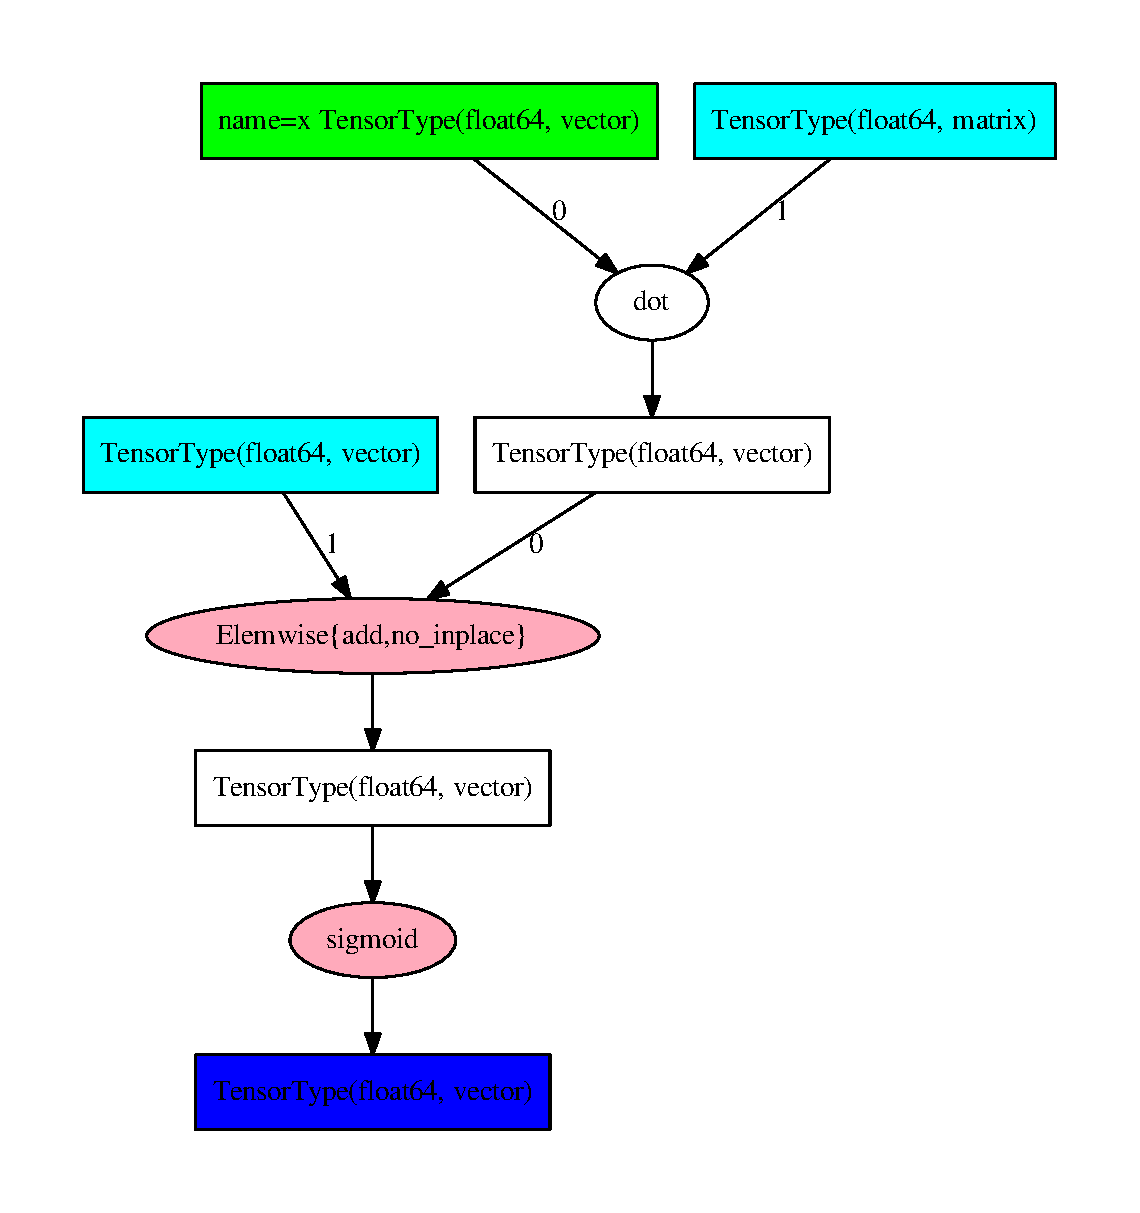
\includegraphics[height=0.9\textheight]{pydotprint_out_long.pdf}
\end{frame}

\begin{frame}{\texttt{pydotprint(out)}}
    \center
    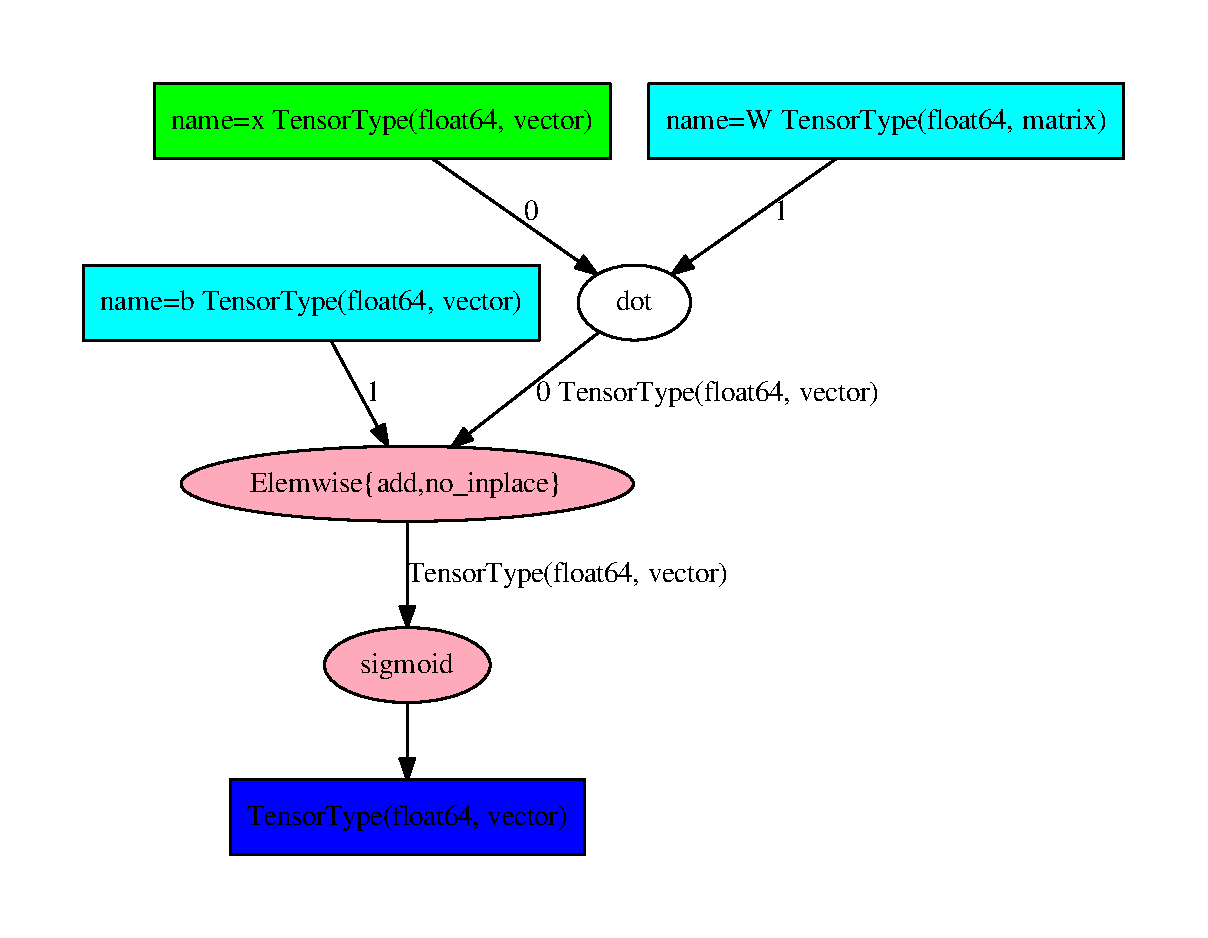
\includegraphics[height=0.9\textheight]{pydotprint_out.pdf}
\end{frame}

\subsection{Deriving gradients}
\begin{frame}{The back-propagation algorithm}
  Application of the chain-rule for functions from ${\mathbb R}^N$ to ${\mathbb R}$.
  \begin{itemize}
    \item $C: {\mathbb R}^N \rightarrow {\mathbb R}$
    \item $f: {\mathbb R}^M \rightarrow {\mathbb R}$
    \item $g: {\mathbb R}^N \rightarrow {\mathbb R}^M$
    \item $C(x) = f(g(x))$
    \item $\left.\frac{\partial C}{\partial x}\right|_x =
              \left.\frac{\partial f}{\partial g}\right|_{g(x)}
              \cdot \left.\frac{\partial g}{\partial x}\right|_x$
  \end{itemize}
  The whole $M \times N$ Jacobian matrix $\left.\frac{\partial g}{\partial x}\right|_x$
  is not needed.

  We only need $\nabla g_x: {\mathbb R}^M \rightarrow {\mathbb R}^N, v \mapsto v \cdot \left.\frac{\partial g}{\partial x}\right|_x$

  This is implemented for (almost) each mathematical operation in Theano.
\end{frame}

\begin{frame}[fragile]{Using \texttt{theano.grad}}
\verb|theano.grad| traverses the graph, applying the chain rule.
  \begin{minted}{python}
dC_dW = theano.grad(C, W)
dC_db = theano.grad(C, b)
# or dC_dW, dC_db = theano.grad(C, [W, b])
  \end{minted}
  \begin{itemize}
    \item \verb|dC_dW| and \verb|dC_db| are symbolic expressions, like \verb|W| and \verb|b|
    \item There are no numerical values at this point
    \item They are part of the same computation graph
    \item They can also be used to build new expressions
  \end{itemize}
  \begin{minted}{python}
upd_W = W - 0.1 * dC_dW
upd_b = b - 0.1 * dC_db
  \end{minted}
\end{frame}

\begin{frame}{\texttt{pydotprint([dC\_dW, dC\_db])}}
    \center
    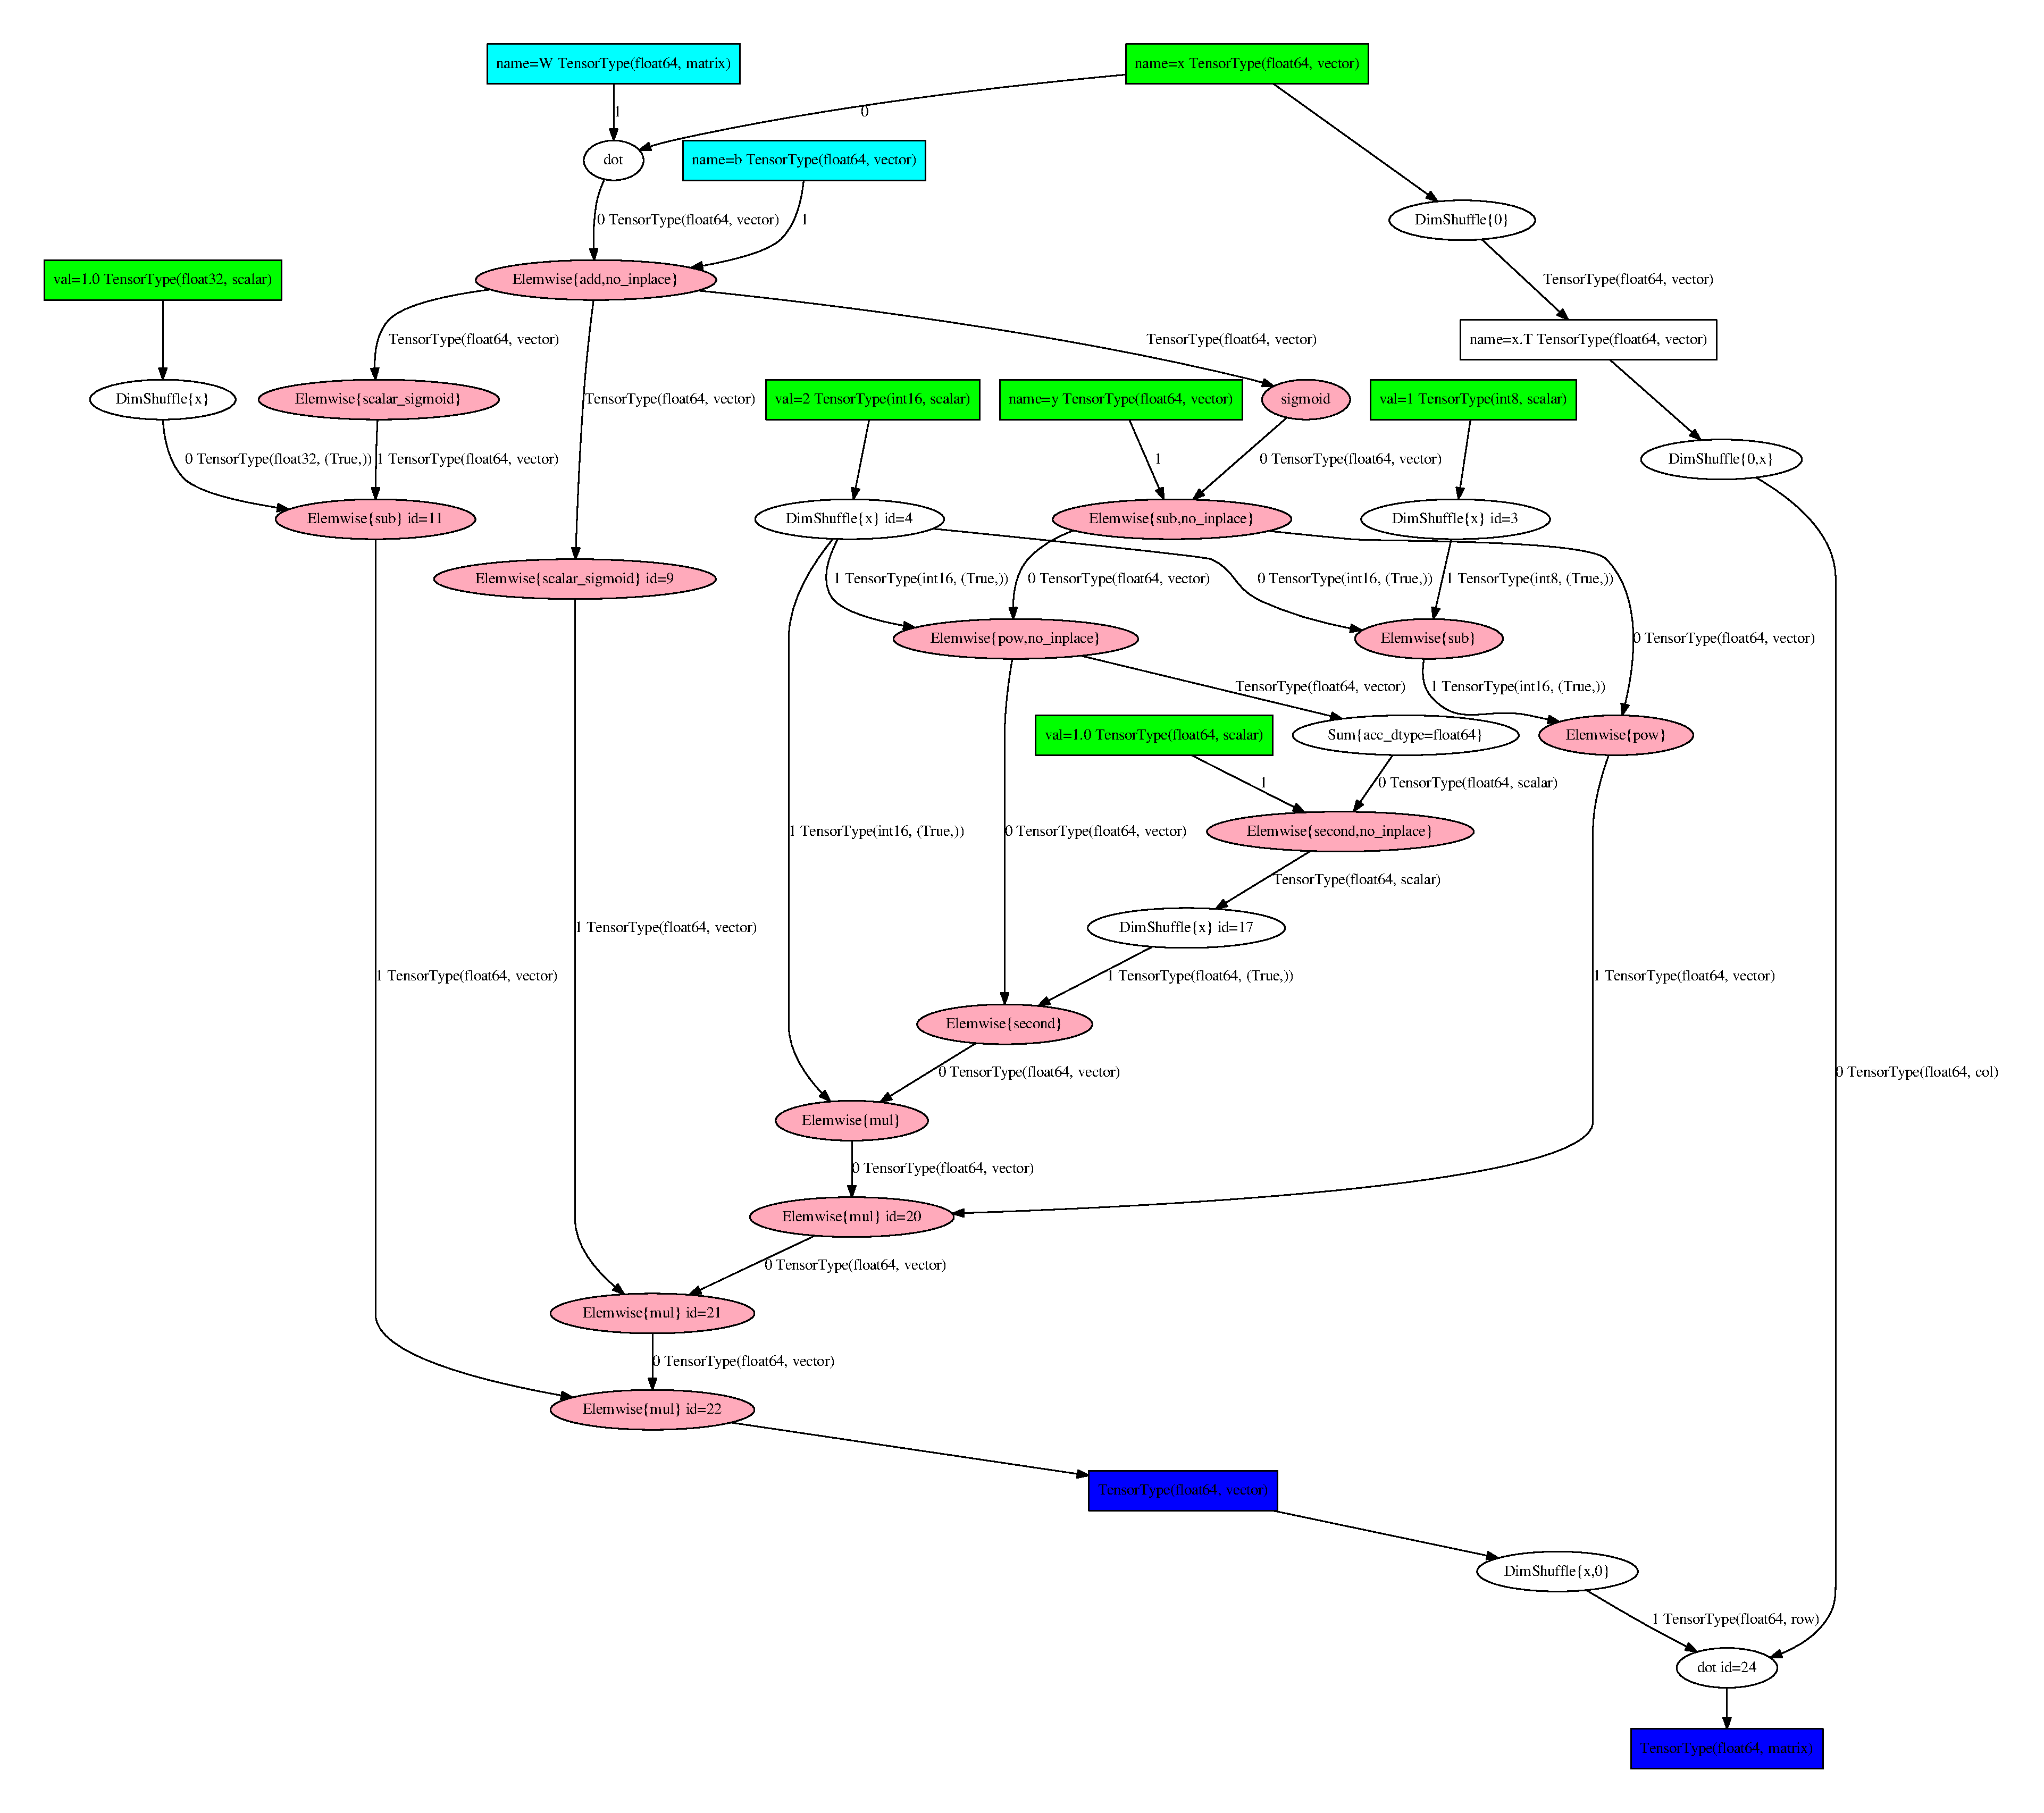
\includegraphics[height=0.9\textheight]{pydotprint_grad.pdf}
\end{frame}

\begin{frame}{\texttt{pydotprint([upd\_W, upd\_b])}}
    \center
    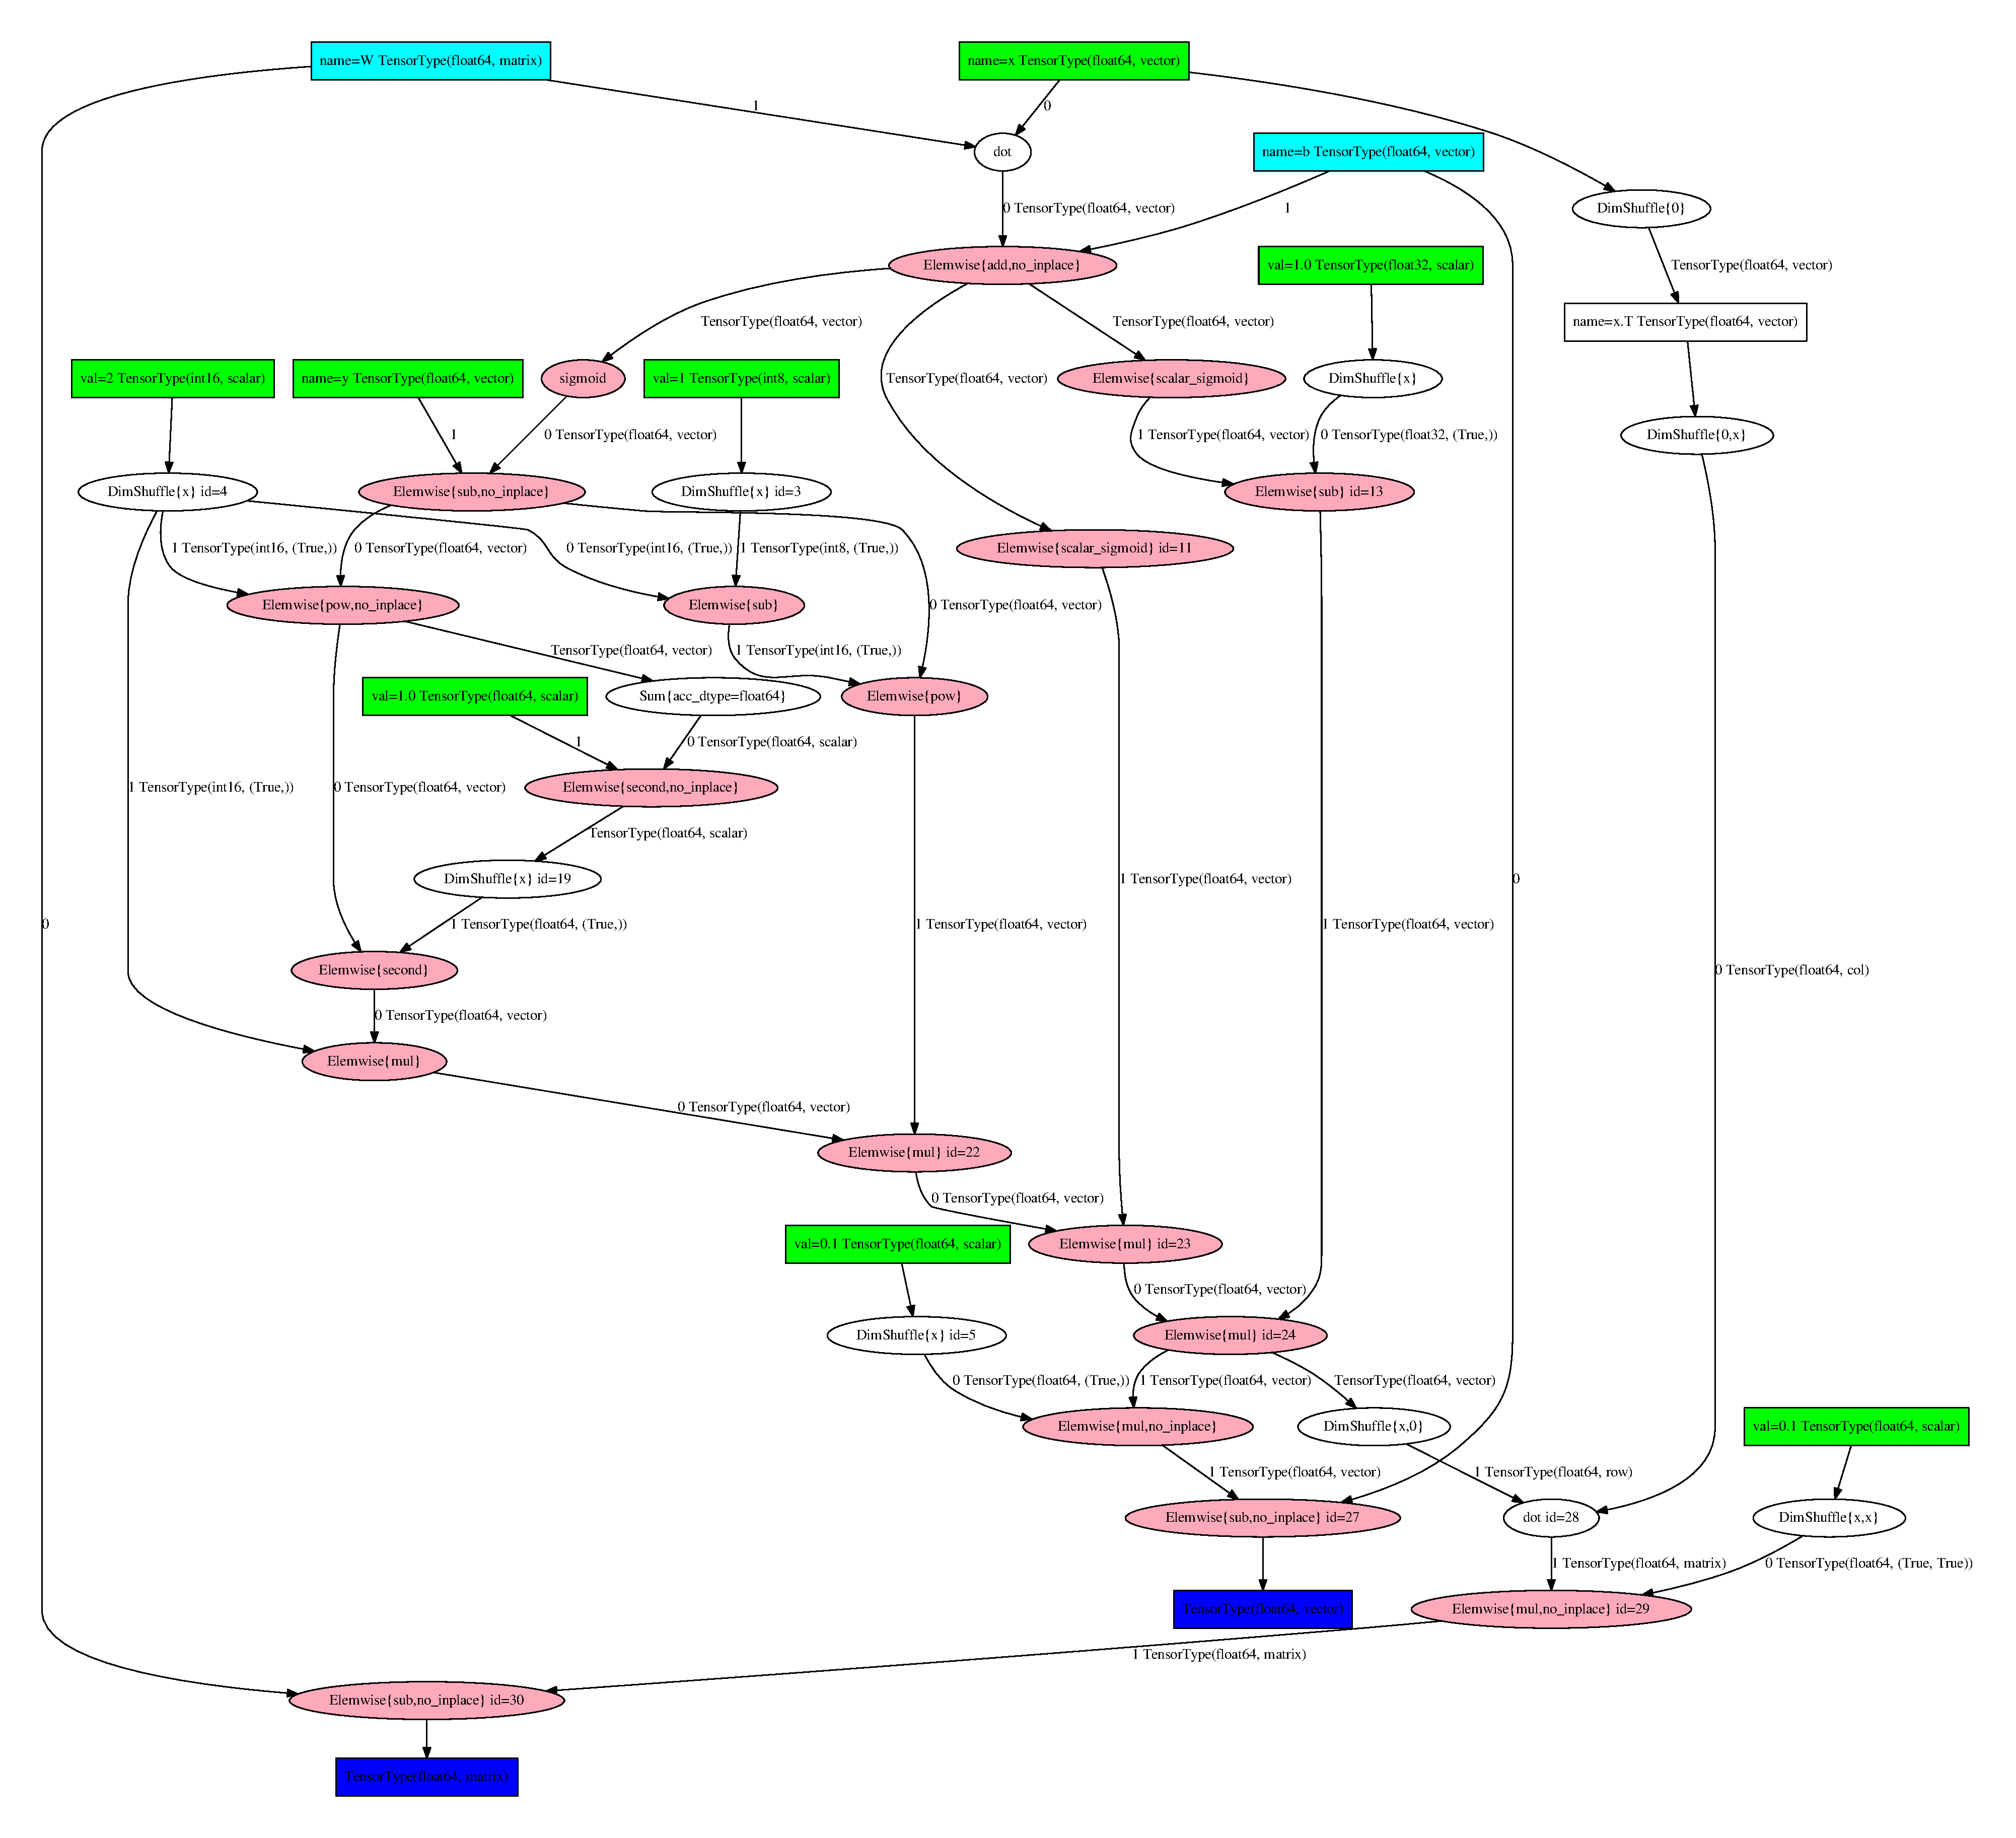
\includegraphics[height=0.9\textheight]{pydotprint_upd.pdf}
\end{frame}


\section{Function compilation}
\begin{frame}
  \tableofcontents[currentsection]
\end{frame}

\subsection{Compiling a Theano function}

\begin{frame}[fragile]{Computing values}
  Build a callable that compute outputs given inputs
  \begin{itemize}
    \item Shared variables are implicit inputs
  \end{itemize}
  \begin{minted}{python}
predict = theano.function([x], out)
x_val = np.random.rand(4)
print(predict(x_val))
# -> array([ 0.9421594 ,  0.73722395,  0.67606977])

monitor = theano.function([x, y], [out, C])
y_val = np.random.uniform(size=3)
print(monitor(x_val, y_val))
# -> [array([ 0.9421594 ,  0.73722395,  0.67606977]),
#     array(0.6191236997823024)]

error = theano.function([out, y], C)
print(error([0.942, 0.737, 0.676], y_val))
# -> array(0.6002210054210885)
  \end{minted}
\end{frame}


\begin{frame}[fragile]{Updating shared variables}
  A function can compute new values for shared variables, and perform updates.
  \begin{minted}{python}
train = theano.function([x, y], C,
                        updates=[(W, upd_W),
                                 (b, upd_b)])
print(b.get_value())
# -> [ 1.  1.  1.]
train(x_val, y_val)
print(b.get_value())
# -> [ 0.9967082   0.99340064  0.97245715]
  \end{minted}
  \begin{itemize}
    \item Variables \verb|W| and \verb|b| are {\bf implicit inputs}
    \item Expressions \verb|upd_W| and \verb|upd_b| are {\bf implicit outputs}
    \item All outputs, including the update expressions, are computed {\bf before} the updates are performed
  \end{itemize}
\end{frame}

\subsection{Graph optimizations}

\begin{frame}{Graph optimizations}
  An optimization replaces a part of the graph with different nodes
  \begin{itemize}
    \item The types of the replaced nodes have to match
    \item The values should be equivalent
  \end{itemize}
  Different goals for optimizations:
  \begin{itemize}
    \item Merge equivalent computations
    \item Simplify expressions: $x / x$ becomes $1$
    \item Numerical stability: ``$\log (1 + x)$'' becomes ``log1p(x)''
    \item Insert in-place an destructive versions of operations
    \item Use specialized, efficient versions (Elemwise loop fusion, BLAS, cuDNN)
    \item Shape inference
    \item Constant folding
    \item Transfer to GPU
  \end{itemize}
\end{frame}

\begin{frame}[fragile]{Enabling/disabling optimizations}
  Trade-off between compilation speed, execution speed, error detection.

  Different pre-defined modes govern the runtime and how much optimizations are applied
  \begin{itemize}
    \item \verb|mode='FAST_RUN'|: default, make the runtime as fast as possible, launching overhead.
      Includes moving computation to GPU if a GPU was selected
    \item \verb|mode='FAST_COMPILE'|: minimize launching overhead, around NumPy speed
    \item \verb|optimizer='fast_compile'|: enables code generation and GPU use, but limits graph optimizations
    \item \verb|mode='DEBUG_MODE'|: checks and double-checks everything, extremely slow
    \item Enable and disable particular optimizations or sets of optimizations
    \item Can be done globally, or for each function
  \end{itemize}

\end{frame}

\subsection{Graph visualization}
\begin{frame}{\texttt{pydotprint(out)}}
    \center
    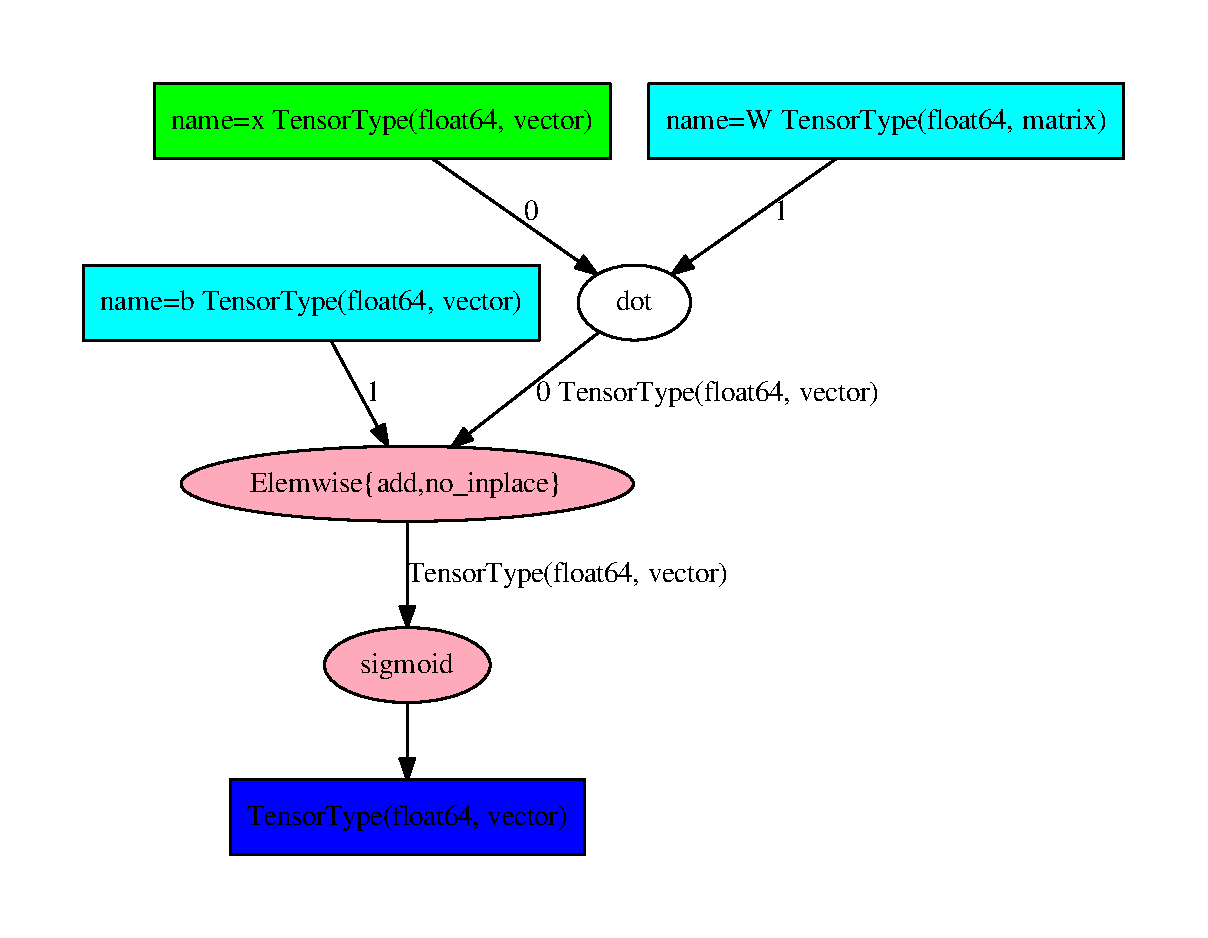
\includegraphics[height=0.9\textheight]{pydotprint_out.pdf}
\end{frame}

\begin{frame}{\texttt{pydotprint(predict)}}
    \center
    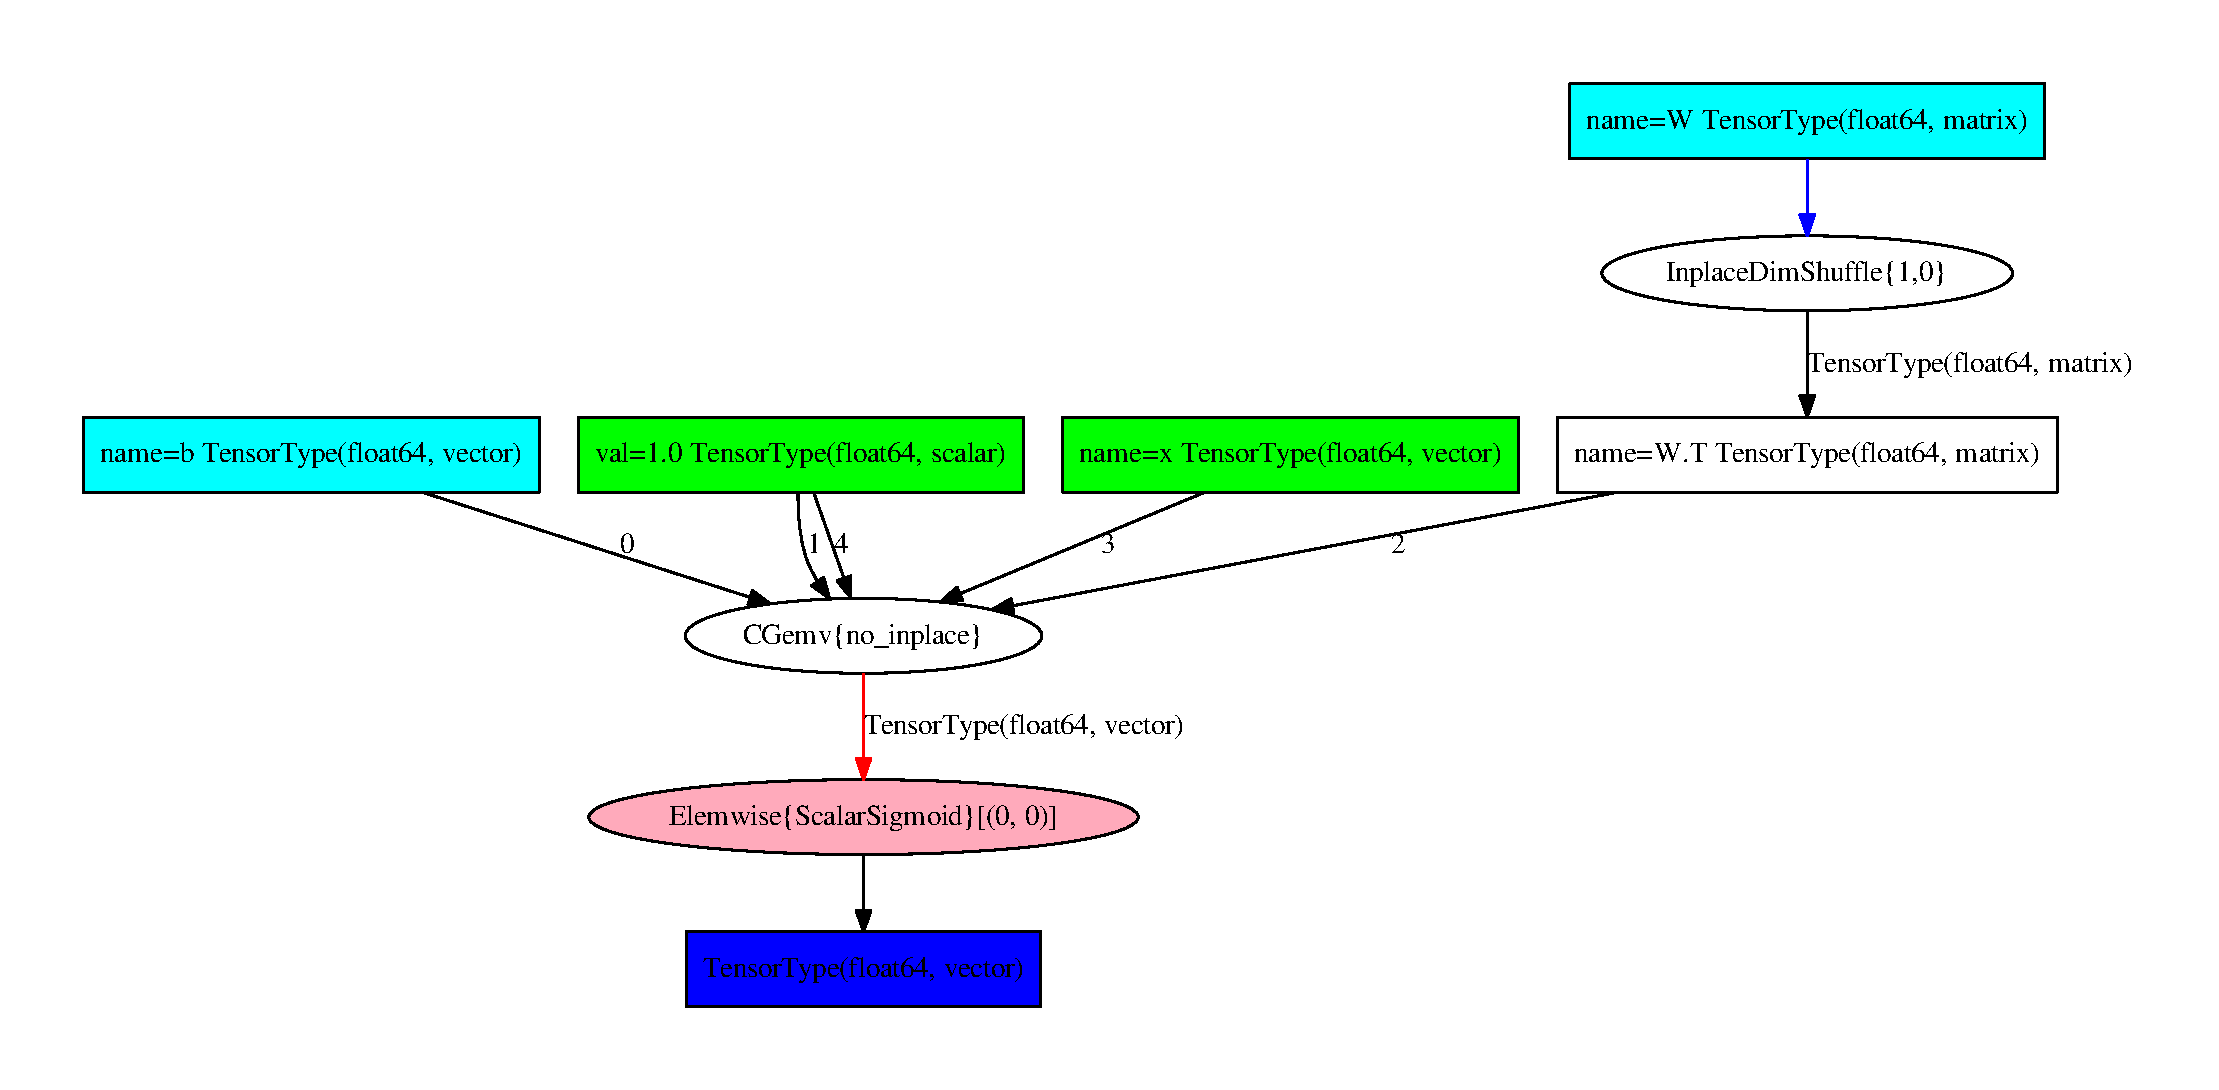
\includegraphics[width=\textwidth]{pydotprint_predict.pdf}
\end{frame}

\begin{frame}{\texttt{pydotprint([upd\_W, upd\_b])}}
    \center
    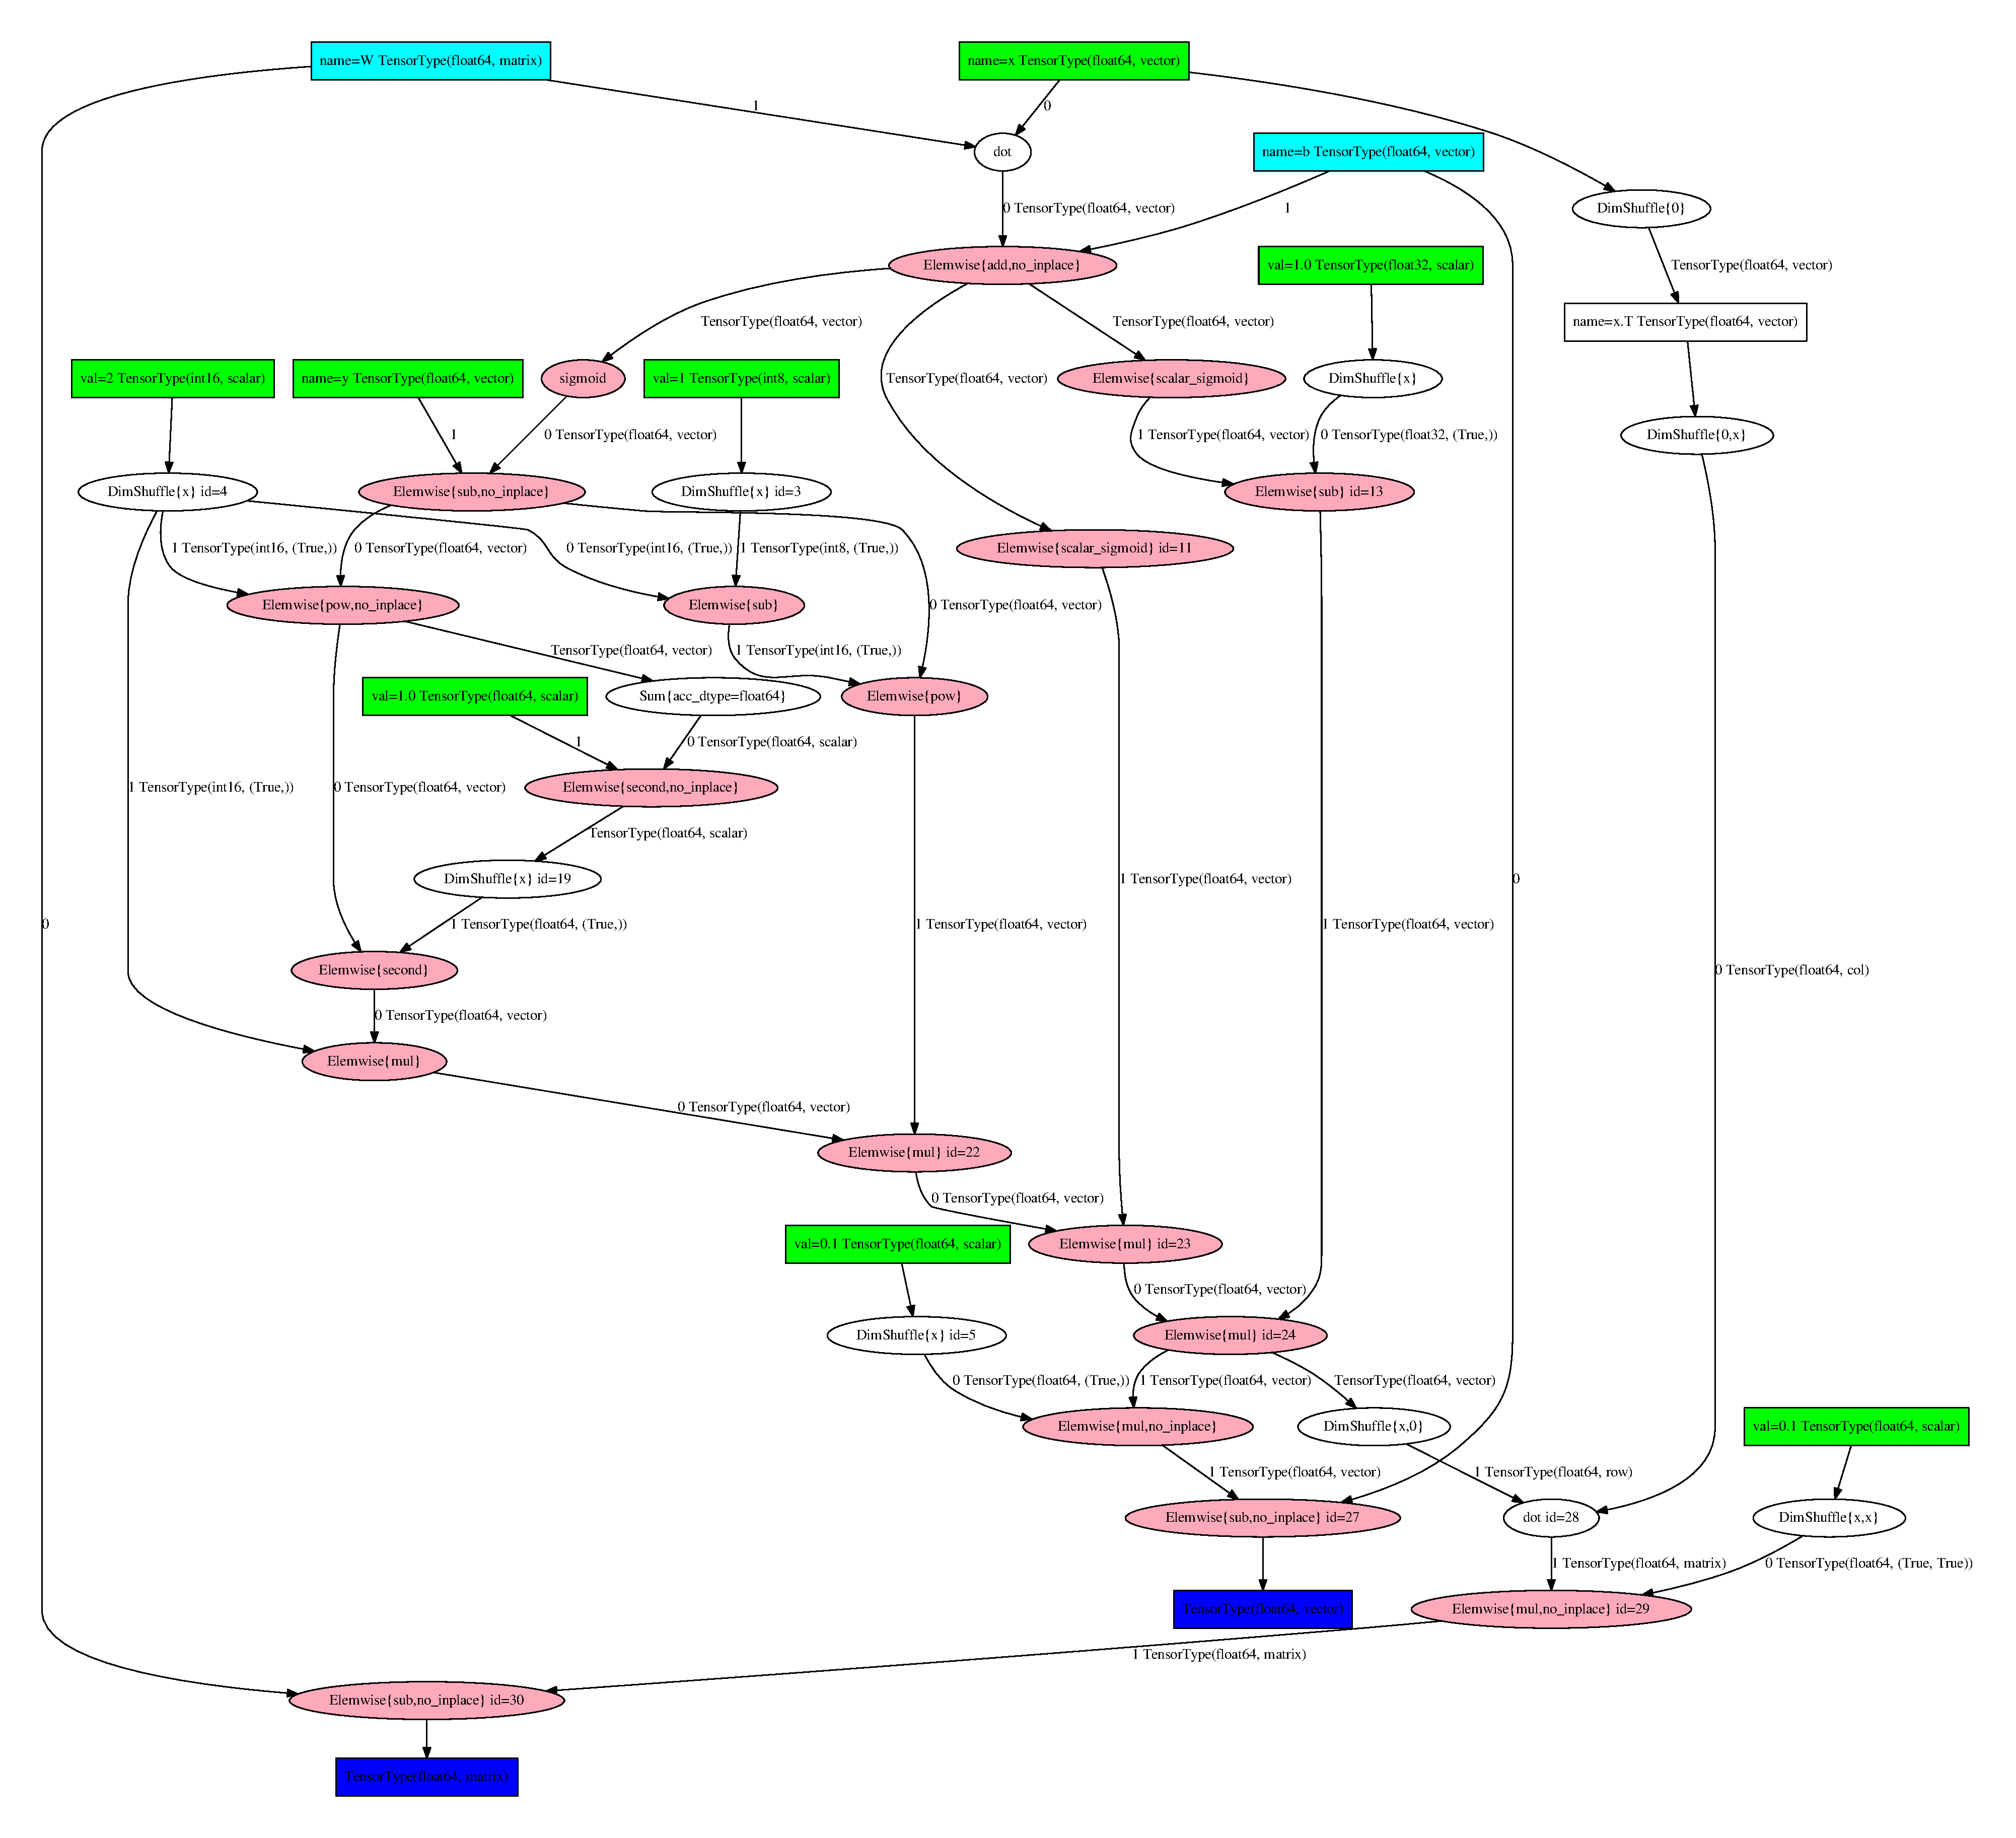
\includegraphics[height=0.9\textheight]{pydotprint_upd.pdf}
\end{frame}

\begin{frame}{\texttt{pydotprint(train)}}
    \center
    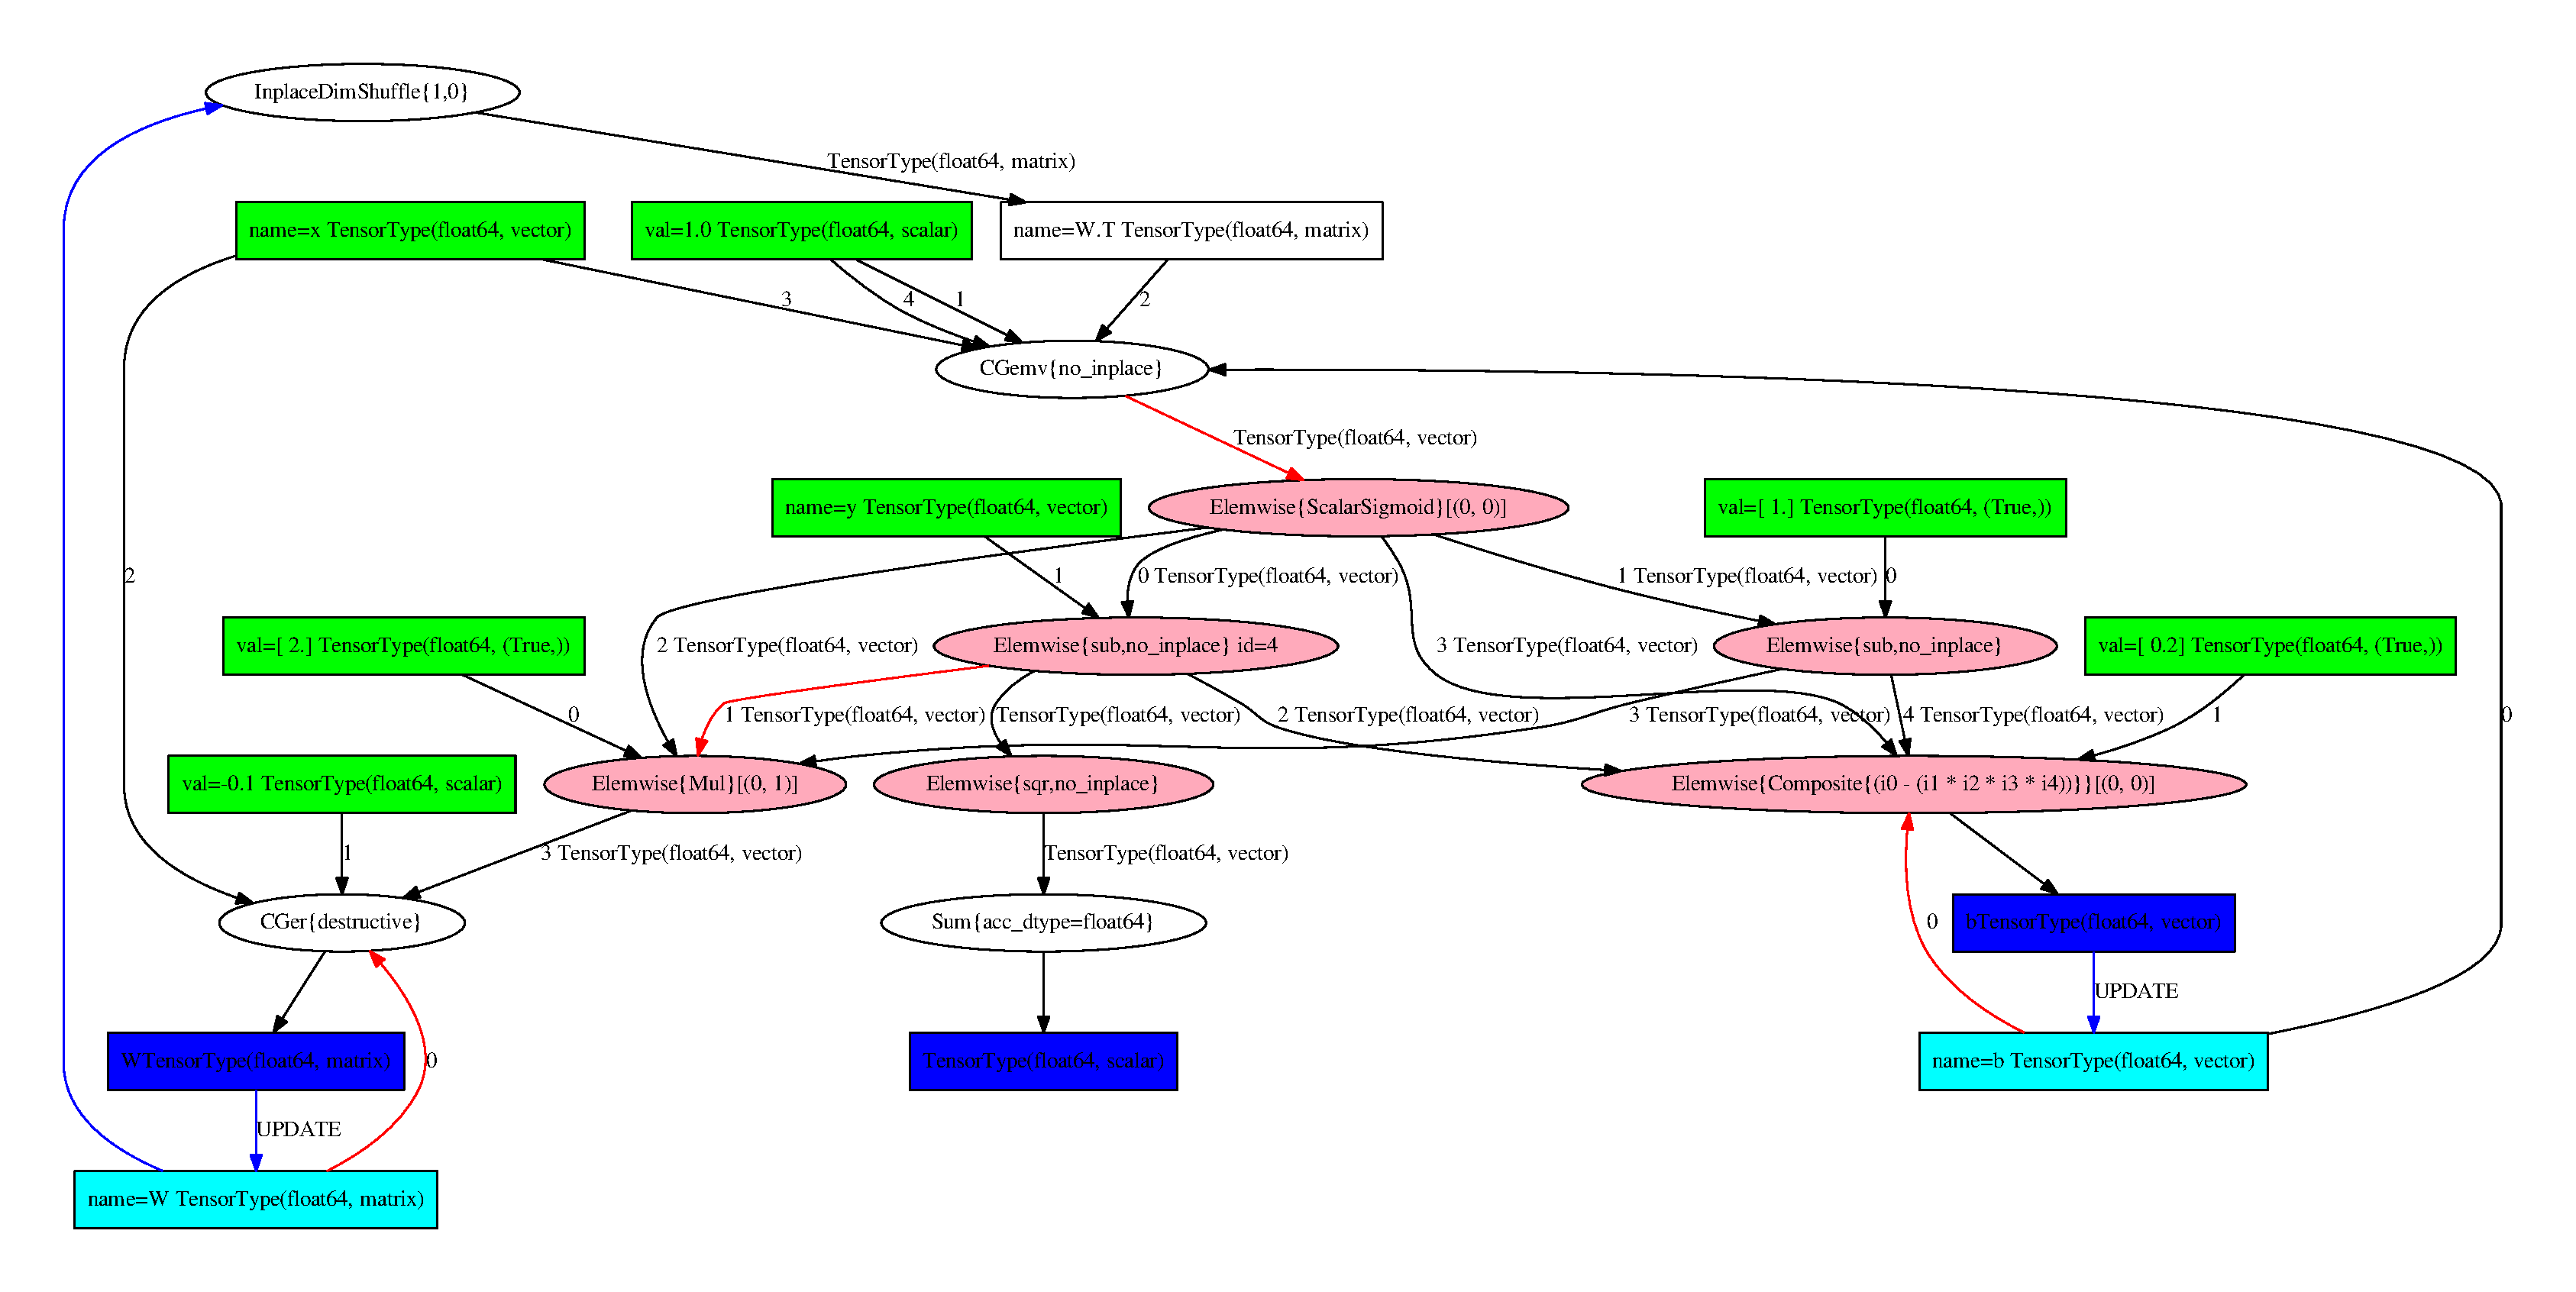
\includegraphics[width=\textwidth]{pydotprint_train.pdf}
\end{frame}


\begin{frame}[fragile]{\texttt{debugprint}}
  \begin{columns}
    \begin{column}{0.45\textwidth}
    \footnotesize
      \begin{verbatim}
debugprint(out)

sigmoid [id A] ''   
 |Elemwise{add,no_inplace} [id B] ''   
   |dot [id C] ''   
   | |x [id D]
   | |W [id E]
   |b [id F]
      \end{verbatim}
    \end{column}

    \begin{column}{0.50\textwidth}
    \footnotesize
      \begin{verbatim}
debugprint(predict)

Elemwise{ScalarSigmoid}[(0, 0)] [id A] ''   2
 |CGemv{no_inplace} [id B] ''   1
   |b [id C]
   |TensorConstant{1.0} [id D]
   |InplaceDimShuffle{1,0} [id E] 'W.T'   0
   | |W [id F]
   |x [id G]
   |TensorConstant{1.0} [id D]
      \end{verbatim}
    \end{column}
  \end{columns}
\end{frame}

%\begin{frame}[fragile]{Graph visualization (2)}
%  \begin{columns}
%    \begin{column}{0.48\textwidth}
%\footnotesize
%      \begin{verbatim}
%theano.printing.debugprint(f)
%CGemv{inplace} [id A] ''   3
% |AllocEmpty{dtype='float64'} [id B] ''   2
% | |Shape_i{1} [id C] ''   1
% |   |W [id D]
% |TensorConstant{1.0} [id E]
% |InplaceDimShuffle{1,0} [id F] 'W.T'   0
% | |W [id D]
% |x [id G]
% |TensorConstant{0.0} [id H]
%
%theano.printing.pydotprint(f)
%      \end{verbatim}
%    \end{column}
%    \begin{column}{0.48\textwidth}
%\footnotesize
%      \begin{verbatim}
%theano.printing.debugprint(g)
%Elemwise{ScalarSigmoid}[(0, 0)] [id A] ''   2
% |CGemv{no_inplace} [id B] ''   1
%   |b [id C]
%   |TensorConstant{1.0} [id D]
%   |InplaceDimShuffle{1,0} [id E] 'W.T'   0
%   | |W [id F]
%   |x [id G]
%   |TensorConstant{1.0} [id D]
%
%theano.printing.pydotprint(g)
%      \end{verbatim}
%    \end{column}
%  \end{columns}
%\end{frame}
%
%\begin{frame}{\tt pydotprint(f)}
%    \includegraphics[width=\textwidth]{pydotprint_f.pdf}
%\end{frame}
%\begin{frame}{\tt pydotprint(g)}
%    \includegraphics[width=\textwidth]{pydotprint_g.pdf}
%\end{frame}
%\begin{frame}{\tt pydotprint(h)}
%    \includegraphics[width=\textwidth]{pydotprint_h.pdf}
%\end{frame}
%
%\begin{frame}[fragile]{\tt d3viz}
%
%{\tt d3viz} enables interactive visualization of graphs in a web browser
%
%  \begin{minted}{python}
%from theano.d3viz import d3viz
%
%d3viz(f, './d3viz_f.html')
%d3viz(g, './d3viz_g.html')
%d3viz(h, './d3viz_h.html')
%  \end{minted}
%\end{frame}

%\begin{frame}[fragile]{Executing a Theano function}
%  Call it with numeric values
%\small
%  \begin{minted}{python}
%import numpy as np
%np.random.seed(42)
%W_val = np.random.randn(4, 3)
%x_val = np.random.rand(4)
%b_val = np.ones(3)
%
%f(x_val, W_val)
%# -> array([ 1.79048354,  0.03158954, -0.26423186])
%
%g(x_val, W_val, b_val)
%# -> array([ 0.9421594 ,  0.73722395,  0.67606977])
%
%h(x_val, W_val, b_val)
%# -> [array([ 1.79048354,  0.03158954, -0.26423186]),
%#     array([ 0.9421594 ,  0.73722395,  0.67606977])]
%
%i(x_val, W_val, b_val)
%# -> [array([ 2.79048354,  1.03158954,  0.73576814]),
%#     array([ 0.9421594 ,  0.73722395,  0.67606977])]
%  \end{minted}
%\end{frame}

%\section{Graph definition and Syntax}
%\begin{frame}
%  \tableofcontents[currentsection]
%\end{frame}
%
%\subsection{Graph structure}
%\begin{frame}[fragile]{Graph structure}
%  The graph that represents mathematical operations is {\bf bipartite},
%  and has two sorts of nodes:
%  \begin{itemize}
%    \item \verb|Variable| nodes, or variables, that represent {\em data}
%    \item \verb|Apply| nodes, that represent the application of
%      {\em mathematical operations}
%  \end{itemize}
%  In practice:
%  \begin{itemize}
%    \item Variables are used for the graph inputs and outputs, and intermediate values
%    \item Variables will hold data during the function execution phase
%    \item An Apply node has inputs and outputs, which are variables
%    \item An Apply node represents the specific application of an Op on these input variables
%    \item The same variable can be used as inputs by several Apply nodes
%  \end{itemize}
%\end{frame}
%
%\begin{frame}
%  \center
%  \includegraphics[width=0.6\textwidth]{apply.pdf}
%\end{frame}

%\begin{frame}{\tt pydotprint(f, compact=False)}
%    \includegraphics[width=\textwidth]{pydotprint_f_notcompact.pdf}
%\end{frame}

%\subsection{Strong typing}
%\begin{frame}{Strong typing}
%  \begin{itemize}
%    \item All Theano variables have a type
%    \item Different categories of types. Most used:
%      \begin{itemize}
%        \item TensorType for NumPy ndarrays
%        \item GpuArrayType for CUDA arrays (CudaNdarrayType in the old back-end)
%        \item Sparse for scipy.sparse matrices
%      \end{itemize}
%    \item ndim, dtype, broadcastable pattern are part of the type
%    \item shape and memory layout (strides) are {\bf not}
%  \end{itemize}
%\end{frame}

%\begin{frame}[fragile]{Broadcasting tensors}
%  \begin{itemize}
%    \item Implicit replication of arrays along broadcastable dimensions
%    \item Broadcastable dimensions will {\bf always} have length 1
%    \item Such dimensions can be added to the left
%  \end{itemize}
%  \begin{minted}{python}
%r = T.row('r')
%print(r.broadcastable)  # (True, False)
%c = T.col('c')
%print(c.broadcastable)  # (False, True)
%
%f = theano.function([r, c], r + c)
%print(f([[1, 2, 3]], [[.1], [.2]]))
%# [[ 1.1  2.1  3.1]
%#  [ 1.2  2.2  3.2]]
%  \end{minted}
%\end{frame}

%%% ???
%\subsection{Differences from Python/NumPy}
%\begin{frame}[fragile]{No side effects}
%  Create new variables, cannot \emph{change} them
%  \begin{itemize}
%    \item \verb|a += 1| works, returns new variable and re-assign
%    \item \verb|a[:] += 1|, or \verb|a[:] = 0| do \textbf{not} work
%      (the \verb|__setitem__| method cannot return a new object)
%    \item \verb|a = T.inc_subtensor(a[:], 1)| or \verb|a = T.set_subtensor(a[:], 0)|
%    \item This will create a new variable, and re-assign a to it
%    \item Theano will figure out later if it can use an in-place version
%  \end{itemize}
%  Exceptions:
%  \begin{itemize}
%    \item The \verb|Print()| Op
%    \item The \verb|Assert()| Op
%    \item You have to re-assign (or use the returned value)
%    \item These can disrupt some optimizations
%      %TODO: example
%  \end{itemize}
%\end{frame}
%
%\begin{frame}[fragile]{Python keywords}
%  We cannot redefine Python's keywords: they affect the flow when building the graph, not when executing it.
%  \begin{itemize}
%    \item \verb|if var:| will always evaluate to \verb|True|.
%      Use \verb|theano.ifelse.ifelse(var, expr1, expr2)|
%    \item \verb|for i in var:| will not work if \verb|var| is symbolic.
%      If \verb|var| is numeric: loop unrolling. You can use \verb|theano.scan|.
%    \item \verb|len(var)| cannot return a symbolic shape, you can use
%      \verb|var.shape[0]|
%    \item \verb|print| will print an identifier for the symbolic variable,
%      there is a \verb|Print()| operation
%  \end{itemize}
%\end{frame}

%%% ???
%\section{Graph Transformations}
%\begin{frame}
%  \tableofcontents[currentsection]
%\end{frame}
%
%\subsection{Substitution and Cloning}
%\begin{frame}[fragile]{The {\tt givens} keyword}
%  With the variables defined earlier:
%  \begin{minted}{python}
%x = T.vector('x')
%W = T.matrix('W')
%b = T.vector('b')
%dot = T.dot(x, W)
%out = T.nnet.sigmoid(dot + b)
%  \end{minted}
%
%  Substitution at the last moment, when compiling a function
%  \begin{minted}{python}
%x_ = T.vector('x_')
%x_n = (x_ - x_.mean()) / x_.std()
%f_n = theano.function([x_, W], dot, givens={x: x_n})
%f_n(x_val, W_val)
%# -> array([ 1.90651511,  0.60431744, -0.64253361])
%  \end{minted}
%\end{frame}
%
%\begin{frame}[fragile]{Cloning with replacement}
%  Useful when building the expression graph
%  \begin{minted}{python}
%dot_n, out_n = theano.clone(
%    [dot, out],
%    replace={x: (x - x.mean()) / x.std()})
%f_n = theano.function([x, W], dot_n)
%f_n(x_val, W_val)
%# -> array([ 1.90651511,  0.60431744, -0.64253361])
%  \end{minted}
%\end{frame}


%\begin{frame}{\tt pydotprint(cost\_and\_upd)}
%  \includegraphics[width=\textwidth]{pydotprint_cost_and_upd.pdf}
%\end{frame}
%
%\subsection{Shared variables}
%\begin{frame}[fragile]{Update values}
%  Simple ways to update values
%  \begin{minted}{python}
%C_val, dC_dW_val, dC_db_val = cost_and_grads(x_val, W_val, b_val, y_val)
%W_val -= 0.1 * dC_dW_val
%b_val -= 0.1 * dC_db_val
%
%C_val, W_val, b_val = cost_and_upd(x_val, W_val, b_val, y_val)
%  \end{minted}
%  \begin{itemize}
%    \item Cumbersome
%    \item Inefficient: memory, GPU transfers
%  \end{itemize}
%\end{frame}

%\begin{frame}{Shared variables}
%  \begin{itemize}
%    \item Symbolic variables, with a {\bf value} associated to them
%    \item The value is {\bf persistent} across function calls
%    \item The value is {\bf shared} among all functions
%    \item The variable has to be an {\bf input variable}
%    \item The variable is an {\bf implicit input} to all functions using it
%  \end{itemize}
%\end{frame}

%\begin{frame}[fragile]{Using shared variables}
%  \begin{minted}{python}
%x = T.vector('x')
%y = T.vector('y')
%W = theano.shared(W_val)
%b = theano.shared(b_val)
%dot = T.dot(x, W)
%out = T.nnet.sigmoid(dot + b)
%f = theano.function([x], dot)  # W is an implicit input
%g = theano.function([x], out)  # W and b are implicit inputs
%print(f(x_val))
%# [ 1.79048354  0.03158954 -0.26423186]
%print(g(x_val))
%# [ 0.9421594   0.73722395  0.67606977]
%  \end{minted}
%  \begin{itemize}
%    \item Use \verb|W.get_value()| and \verb|W.set_value()|
%      to access the value later
%  \end{itemize}
%\end{frame}
%
%\begin{frame}[fragile]{Updating shared variables}
%  \begin{minted}{python}
%C = ((out - y) ** 2).sum()
%dC_dW, dC_db = theano.grad(C, [W, b])
%upd_W = W - 0.1 * dC_dW
%upd_b = b - 0.1 * dC_db
%
%cost_and_perform_updates = theano.function(
%    inputs=[x, y],
%    outputs=C,
%    updates=[(W, upd_W),
%             (b, upd_b)])
%  \end{minted}
%  \begin{itemize}
%    \item Variables \verb|W| and \verb|b| are {\bf implicit inputs}
%    \item Expressions \verb|upd_W| and \verb|upd_b| are {\bf implicit outputs}
%    \item All outputs, including the update expressions, are computed {\bf before} the updates are performed
%  \end{itemize}
%\end{frame}
%
%\begin{frame}{\tt pydotprint(cost\_and\_perform\_updates)}
%  \includegraphics[width=\textwidth]{pydotprint_cost_and_perform_updates.pdf}
%\end{frame}


\section{Optimized execution}
\begin{frame}
  \tableofcontents[currentsection]
\end{frame}

\subsection{Code generation and execution}
\begin{frame}[fragile]{Code generation and execution}
  Code generation for Ops:
  \begin{itemize}
    \item Ops can define C++/CUDA code computing its output values
    \item Dynamic code generation is possible
      \begin{itemize}
        \item For instance, loop fusion for arbitrary sequence of element-wise operations
      \end{itemize}
    \item Code gets compiled into a Python module, cached, and imported
    \item Otherwise, fall back to a Python implementation
  \end{itemize}

  Code execution through a runtime environment, or VM:
  \begin{itemize}
    \item Calls the functions performing computation for the Ops
    \item Deals with ordering constraints, lazy execution
    \item A C++ implementation (CVM) to avoid context switches
      (in/out of the Python interpreter)
  \end{itemize}
\end{frame}

%\begin{frame}[fragile]{The C virtual machine (CVM)}
%  A runtime environment, or VM, that calls the functions performing
%  computation of different parts of the function (from inputs to
%  outputs)
%  \begin{itemize}
%    \item Avoids context switching between C and Python
%    \item Data structure containing
%      \begin{itemize}
%        \item Addresses of inputs and outputs of all nodes (intermediate values)
%        \item Ordering constraints
%        \item Pointer to functions performing the computations
%        \item Information on what has been computed, and needs to be computed
%      \end{itemize}
%    \item Set in advance from Python when compiling a function
%    \item At runtime, if all operations have C code, calling the pointers will be fast
%    \item Also enables lazy evaluation (for \verb|ifelse| for instance)
%  \end{itemize}
%\end{frame}

\subsection{GPU}
\begin{frame}[fragile]{Using the GPU}
  We want to make the use of GPUs as transparent as possible.

  Theano features a new GPU back-end, with
  \begin{itemize}
    \item More dtypes, not only \verb|float32|
    \item Experimental support for \verb|'float16'| for storage
    \item Easier interaction with GPU arrays from Python
    \item Multiple GPUs and multiple streams
    \item \textbf{In the development version only, and future 0.9 release}
  \end{itemize}

  Select GPU by setting the \verb|device| flag to \verb|'cuda'| or \verb|'cuda{0,1,2,...}'|.
  \begin{itemize}
    \item All {\bf shared} variables will be created in GPU memory
    \item Enables optimizations moving supported operations to GPU
    \item You want to make sure to use float32 for speed
  \end{itemize}
\end{frame}

\begin{frame}[fragile]{Configuration flags}
  Configuration flags can be set in a couple of ways:
  \begin{itemize}
    \item In the \verb|.theanorc| configuration file:
      \begin{minted}{text}
[global]
device = cuda0
floatX = float32
      \end{minted}
    \item \verb|THEANO_FLAGS=device=cuda0,floatX=float32| in the shell
    \item In Python:
      \begin{minted}{python}
theano.config.floatX = 'float32'
      \end{minted}
      (\verb|theano.config.device| cannot be set once Theano is imported)
  \end{itemize}
\end{frame}


\section{Advanced Topics}
\begin{frame}
  \tableofcontents[currentsection]
\end{frame}

\subsection{Looping: the \texttt{scan} operation}
\begin{frame}[fragile]{Overview of \texttt{scan}}
  Symbolic looping
  \begin{itemize}
    \item Can perform map, reduce, reduce and accumulate, \ldots
    \item Can access outputs at previous time-step, or further back
    \item Symbolic number of steps
    \item Symbolic stopping condition (behaves as \verb|do ... while|)
    \item Actually embeds a small Theano function
    \item Gradient through \verb|scan| implements backprop through time
    \item Can be transfered to GPU
  \end{itemize}
  We will see a use of \verb|scan| in the LSTM example.
\end{frame}

\begin{frame}[fragile]{Example: Loop with accumulation}
  \footnotesize
    \begin{minted}{python}
k = T.iscalar("k")
A = T.vector("A")

# Symbolic description of the result
result, updates = theano.scan(fn=lambda prior_result, A: prior_result * A,
                              outputs_info=T.ones_like(A),
                              non_sequences=A,
                              n_steps=k)

# We only care about A**k, but scan has provided us with A**1 through A**k.
# Discard the values that we don't care about. Scan is smart enough to
# notice this and not waste memory saving them.
final_result = result[-1]

# compiled function that returns A**k
power = theano.function(inputs=[A, k], outputs=final_result, updates=updates)

print(power(range(10), 2))
# [  0.   1.   4.   9.  16.  25.  36.  49.  64.  81.]
print power(range(10), 4)
# [  0.00000000e+00   1.00000000e+00   1.60000000e+01   8.10000000e+01
#    2.56000000e+02   6.25000000e+02   1.29600000e+03   2.40100000e+03
#    4.09600000e+03   6.56100000e+03]
  \end{minted}
\end{frame}

\subsection{Debugging}
\begin{frame}[fragile]{Visualization, debugging, and diagnostic tools}
  The \emph{definition} of a Theano function is separate from its \emph{execution}.
  To help with this, we provide:
  \begin{itemize}
    \item Information in error messages
    \item Get information at runtime
    \item Monitor NaN or large value
    \item Test values when building the graph
    \item Detect common sources of slowness
    \item Self-diagnostic tools
  \end{itemize}
\end{frame}

\subsection{Extending Theano}

\begin{frame}{Extending Theano}
Theano can be extended in a few different ways
  \begin{itemize}
    \item Creating an Op with Python code
      \begin{itemize}
        \item Easy, using Python bindings for specialized libraries (PyCUDA, \ldots)
        \item Some runtime overhead is possible
        \item Example: 3D convolution using FFT on GPU
      \end{itemize}
    \item Creating an Op with C or CUDA code
      \begin{itemize}
        \item Use the C-API of Python / NumPy / GpuArray, manage refcounts
        \item No overhead of Python function calls, or from the interpreter
        \item C code inline or in a separate file
        \item Example: Caffe-style convolutions, using GEMM, on CPU and GPU
      \end{itemize}
    \item Adding an optimization
      \begin{itemize}
        \item Perform additional graph simplifications
        \item Replace part of the graph by a new optimized Op
      \end{itemize}
  \end{itemize}
\end{frame}

%\begin{frame}[fragile]{The easy way: Python}
%\small
%  Easily wrap Python code, specialized library with Python bindings (PyCUDA, \ldots)
%
%  \begin{minted}{python}
%import theano
%import numpy
%from theano.compile.ops import as_op
%
%def infer_shape_numpy_dot(node, input_shapes):
%    ashp, bshp = input_shapes
%    return [ashp[:-1] + bshp[-1:]]
%
%@as_op(itypes=[theano.tensor.fmatrix, theano.tensor.fmatrix],
%       otypes=[theano.tensor.fmatrix], infer_shape=infer_shape_numpy_dot)
%def numpy_dot(a, b):
%   return numpy.dot(a, b)
%
%  \end{minted}
%  \begin{itemize}
%    \item Overhead of Python call could be slow
%    \item To define the gradient, have to actually define a class deriving from \verb|Op|,
%      and define the \verb|grad| method.
%  \end{itemize}
%  Has been used to implement 3D convolution using FFT on GPU
%\end{frame}
%
%\begin{frame}[fragile]{The harder way: C code}
%  \begin{itemize}
%    \item Understand the C-API of Python / NumPy / CudaNdarray
%    \item Handle arbitrary strides (or use \verb|GpuContiguous|)
%    \item Manage refcounts for Python
%    \item No overhead of Python function calls, or from the interpreter (if garbage
%      collection is disabled)
%    \item Now easier: C code in a separate file
%  \end{itemize}
%  New contributors wrote Caffe-style convolutions, using GEMM, on CPU and GPU that way.
%
%  For more about this, see Arnaud's tutorial on Sept. 28th.
%\end{frame}

\subsection{New features}
\begin{frame}[fragile]{Features recently added to Theano}
  \begin{itemize}
    \item New GPU back-end (dev branch), with:
      \begin{itemize}
        \item Arrays of all dtypes, half-precision float (\verb|float16|) for storage
        \item Support for multiple GPUs in the same function
      \end{itemize}
    \item Performance improvements
      \begin{itemize}
        \item Better interface and implementations for convolution and transposed convolution
        \item Integration of CuDNN (now v5) for 2D/3D convolutions and pooling
        \item CNMeM and a similar allocator for GPU memory
        \item Data-parallelism with Platoon (\url{github.com/mila-udem/platoon/})
      \end{itemize}
    \item Faster graph optimization phase
      \begin{itemize}
        \item Execution of un-optimized graph on GPU (quicker compile time)
        \item Various ways to avoid recompilation
      \end{itemize}
    \item New diagnostic tools
      \begin{itemize}
        \item Interactive visualization (d3viz)
        \item \verb|PdbBreakPoint|
      \end{itemize}
  \end{itemize}
\end{frame}

\begin{frame}[fragile]{What to expect in the near future}
  \begin{itemize}
    \item Better support for int operations on GPU (indexing, argmax)
    \item More CuDNN operations (basic RNNs, batch normalization)
    \item Better support for 3D convolution / pooling
    \item Simpler, faster optimization mode
    \item Data-parallelism across nodes in Platoon
  \end{itemize}
\end{frame}


\section{}

\begin{frame}{Acknowledgements}
  \begin{itemize}
    \item All people working or having worked at the MILA (previously LISA), especially Theano contributors
      \begin{itemize}
        \item
          Frédéric Bastien,
          Yoshua Bengio,
          James Bergstra,
          Arnaud Bergeron,
          Philemon Brakel,
          Olivier Breuleux,
          Pierre Luc Carrier,
          Mathieu Germain,
          Ian Goodfellow,
          Simon Lefrançois,
          Razvan Pascanu,
          Joseph Turian,
          David Warde-Farley,
          and many more
      \end{itemize}
    \item Compute Canada, Calcul Québec, NSERC, the Canada Research Chairs, and CIFAR for providing funding or access to compute resources
    \item Stanford AI Lab and the organizers of the Deep Learning School
  \end{itemize}
\end{frame}

\begin{frame}[fragile]{Thanks for your attention}
  \uncover<1->{%
    Questions, comments, requests?
  }
  \vspace{.5cm}

  \uncover<2->{%
    \url{github.com/lamblin/bayareadlschool/}
    \begin{itemize}
      \item Slides: {\tt intro\_theano.pdf}
      \item Companion notebook: {\tt intro\_theano.ipynb}
    \end{itemize}
  }

  \vspace{.5cm}
  \uncover<3->{%
    More resources
    \begin{itemize}
      \item Documentation: \url{deeplearning.net/software/theano/}
      \item Code: \url{github.com/Theano/Theano/}
      \item Article: The Theano Development Team, ``Theano: A Python framework for fast computation of mathematical expressions'', \url{arxiv.org/abs/1605.02688}
      \item Deep Learning Tutorials: \url{deeplearning.net/tutorial/}
    \end{itemize}
  }
\end{frame}

\begin{frame}[fragile]{Examples}
  Tutorial repository on GitHub:\\
  \url{github.com/lamblin/bayareadlschool/}

  \begin{itemize}
    \item Install the dependencies
    \item Clone the repository
      \begin{minted}[fontfamily=tt]{bash}
git clone https://github.com/lamblin/bayareadlschool.git
      \end{minted}
    \item Launch the notebook
      \begin{minted}[fontfamily=tt]{bash}
jupyter notebook bayareadlschool
      \end{minted}
    \item Navigate to {\tt convnet}, then {\tt exercises.ipynb}
    \item Navigate to {\tt lstm}, then {\tt exercises.ipynb}
  \end{itemize}
\end{frame}
\end{document}
